\chapter{\IfLanguageName{dutch}{Training van het model}{Training the model}}
\label{ch:trainingvhmodel}
Voordat het model gebruikt kan worden moet het eerst getraind worden.
Dit gebeurt door het model te voeden met een dataset van video's en hun bijhorende uitkomsten.
Bij dit model is de dataset al reeds gepreprocessed en in een formaat dat het model kan gebruiken.
Dit is echter nadelig voor ons omdat we niet weten hoe de data is gepreprocessed.
Waardoor het bij de inferentie moeilijker is om de data te pre-processen.

\section{Dataset}
\label{sec:dataset}

De dataset die gebruikt wordt is de \textit{RWTH-PHOENIX-Weather 2014 T} \footnote{\url{https://www-i6.informatik.rwth-aachen.de/~koller/RWTH-PHOENIX-2014-T/}} dataset.
Dit is een veelgebruikte dataset voor het trainen van gebarentaalmodellen.
De dataset bevat video's van het Duits gebarentaal en hun bijhorende transcripties.
De video's zijn extracties van het weerbericht van de Duitse publieke omroep PHOENIX.
\\
\\
De reden voor een Duitse dataset is omdat in het Vlaams gebarentaal geen goed genoege dataset bestaat.
Deze dataset wordt ook meestal gebruikt als benchmark voor gebarentaalmodellen.
Dit is samen met de RWTH-PHOENIX-Weather 2014\footnote{\url{https://www-i6.informatik.rwth-aachen.de/~koller/RWTH-PHOENIX/}} dataset en de CSL-Daily\footnote{\url{https://ustc-slr.github.io/datasets/2021_csl_daily/}} dataset de meest voorkomende dataset om gebarentaalmodellen te testen.
\\
\\
De github van het model geeft echter een link naar een kleinere subset van de dataset.
Het SignFormer model is gebouwd om met deze subset te werken en niet met de volledige dataset.
De precieze manier waarop de dataset is gepreprocessed is te vinden in een totaal andere paper namelijk:\textcite{SLTS}.
Echter staat hier ook niet exact uitgelegd hoe de data is gepreprocessed.
Er kan wel een schatting gemaakt worden van hoe de data is gepreprocessed.
Deze schatting wordt dan ook effectief gebruikt in de inferentie.


\section{Training}
\label{sec:training}
Voor het trainen van het model is er een aantal hyperparameters ingesteld.
De hyperparameters zijn:
\begin{itemize}
  \item Feature size: 1024
  \item Learning rate: 0.0004
  \item Epochs: 1000
  \item Max Sentence Length: 400
  \item Eval metric: bleu
  \item Batch size: 32
  \item Early stopping: eval metric
  \item translation beam sizes: 1, ..., 10
  \item translation beam alpha's: -1, ..., 5
\end{itemize}

De ingestelde hyperparameters definiëren belangrijke aspecten van het trainingsproces en de architectuur van het model voor gebarentaalherkenning. 
De 'Feature size' van 1024 bepaalt de dimensionaliteit van de feature vectoren die worden geëxtraheerd uit de input data (zoals videoframes of sequenties die gebaren vertegenwoordigen). 
Deze vector van 1024 elementen representeert de kenmerken (visuele aspecten, beweging) van de input op een bepaald moment of segment, die relevant zijn voor het herkennen van het gebaar. 
Een hogere waarde staat toe complexere visuele of temporele kenmerken vast te leggen.
De keuze voor 1024 hangt dus af van het formaat van de voorverwerkte dataset.
\\
De 'Learning rate' van 0.0004 is een cruciale parameter voor de optimalisatie: het bepaalt de stapgrootte waarmee de gewichten van het model aangepast worden tijdens het leren. 
Een kleine waarde zoals 0.0004 zorgt vaak voor stabiele convergentie.
\\
Het aantal 'Epochs' is ingesteld op 1000, wat aangeeft dat het model potentieel 1000 keer de gehele trainingsdataset doorloopt. 
Echter, door gebruik te maken van 'Early stopping', zal de training waarschijnlijk eerder stoppen om overfitting te voorkomen.
\\
'Early stopping' is geconfigureerd om te reageren op de 'Eval metric', wat betekent dat de training stopt zodra de prestatie op de validatieset, gemeten met de 'bleu' score, niet meer verbetert. 
Het gebruik van 'bleu' (Bilingual Evaluation Understudy) als evaluatiemetriek suggereert dat het model mogelijk getraind wordt voor gebarentaal vertaling naar tekst, aangezien BLEU een veelgebruikte metriek is voor het evalueren van de kwaliteit van gegenereerde tekst.
\\
De 'Max Sentence Length' van 400 specificeert de maximale lengte van de inputsequenties in termen van tijdstappen of frames. 
Dit is dus de maximale duur van een gebaar of een reeks gebaren die het model in één keer kan verwerken. 
Langere sequenties worden typisch afgekapt en kortere worden aangevuld (padding).
\\
Tot slot definieert de 'Batch size' van 32 het aantal trainingsvoorbeelden (oftewel sequenties van gebarendata) dat gezamenlijk door het model wordt verwerkt in één iteratie voordat de modelgewichten worden bijgewerkt. 
Samen bepalen deze parameters hoe het model leert en presteert op de gebarentaalherkenningstaak.

\subsubsection{Andere training parameters}
Naast de hyperparameters zijn er ook andere parameters ingesteld voor het trainen van het model.
Dit zijn vooral parameters voor het model zelf.
De parameters zijn:
\begin{itemize}
  \item encoder
  \begin{itemize}
    \item layers: 1
    \item type: transformer
    \item attention heads: 8
    \item embeddings size: 256
    \item activation: softsign
  \end{itemize}
  \item decoder
  \begin{itemize}
    \item layers: 1
    \item type: transformer
    \item attention heads: 8
    \item embeddings size: 256
    \item activation: softsign
  \end{itemize}
\end{itemize}

De parameters zijn ingesteld om de architectuur van het model te definiëren.
De encoder en decoder zijn beide transformer-gebaseerd, wat betekent dat ze gebruik maken van self-attention mechanismen om de relaties tussen verschillende delen van de inputsequentie te begrijpen.


\section{Resultaten}
\label{sec:results}
Na het trainen van het model zijn er verschillende evaluaties uitgevoerd om de prestaties van het model te meten.
Deze evaluaties zijn gemaakt op een computer met een NVIDIA GeForce RTX 3050 Laptop GPU en een RAM van 32 GB.
De training heeft in totaal \textbf{153 epochs} geduurd.
En een tijd van \textbf{1u en 12 minuten} in beslag genomen.
En heeft ongeveer \textbf{3,88 miljoen parameters} of ook wel een grootte van \textbf{15,5 MB}.
Dit is een relatief klein model in vergelijking met andere modellen.
Dit is voordat er enige optimalisaties voor een edge device zijn toegepast.
Het model heeft twee vocabulaires gemaakt.
De gloss vocabulary is voor aan elk gebaar een betekenis te geven.
De tekst vocabulary is voor de betekenis van de gebaren in een vloeiende tekst te zetten.
De gloss vocabulary heeft \textbf{1087 verschillende gebaren}.
Terwijl de tekst vocabulary \textbf{2889 verschillende woorden} heeft.
\\
\\
Het model heeft ook de 'Beam Size' en 'Alpha' parameters geoptimaliseerd.
De 'Beam Size' parameter bepaalt het aantal mogelijke vertalingen dat het model overweegt bij het genereren van de output.
De 'Alpha' parameter is een gewichtsparameter die de invloed van de lengte van de output op de uiteindelijke score beïnvloedt.
Deze zijn een beam size van 10 en een alpha van 2.
Het finaal model is getraind met een beam size van 10 en een alpha van 2.
Hierbij heeft het beste versie van het model volgende scores behaald:
\begin{table}[h]
  \begin{tabular}{ |l||c|c| |}
    \hline
    & Development Set & Test Set \\
    \hline
    BLUE-1 & 45.04 & 45.92 \\
    \hline
    BLUE-2 & 32.53 & 33,05 \\
    \hline
    BLUE-3 & 25.33 & 26,78 \\
    \hline
    BLUE-4 & 20.63 & 22.11 \\
    \hline
    BLUE-L & 20.63 & 22.11 \\
    \hline
    CHRF & 43.51 & 44.73 \\
    \hline
    ROUGE & 46.83 & 47.24 \\
    \hline
  \end{tabular}
  \caption{Resultaten van het SignFormer model}
  \label{tab:results-training}
\end{table}
Deze resultaten zijn behaald op de testset en developmentset van de dataset.
De belangrijke resultaten zijn die op de testset.
Je kan zien dat de scores van de testset en developmentset dicht bij elkaar liggen.
Dit is een goed teken dat het model niet overfit is op de training data.\\
De BLUE score (Zie figuur \ref{fig:blue-scores}) is een maat voor de kwaliteit van de gegenereerde tekst in vergelijking met de referentietekst.\\
De CHRF score (Zie figuur \ref{fig:rouge-scores}) is een maat voor de kwaliteit van de gegenereerde tekst in vergelijking met de referentietekst, maar is meer gericht op de karakters in plaats van de woorden.\\
De ROUGE score (Zie figuur \ref{fig:chrf-scores}) is een maat voor de kwaliteit van de gegenereerde tekst in vergelijking met de referentietekst, maar is meer gericht op de zinnen in plaats van de woorden.\\

\begin{figure}[p!] % Probeer deze figuren samen op een aparte float page te plaatsen
    \centering % Centreer de figuren horizontaal op de pagina

    % Eerste figuur
    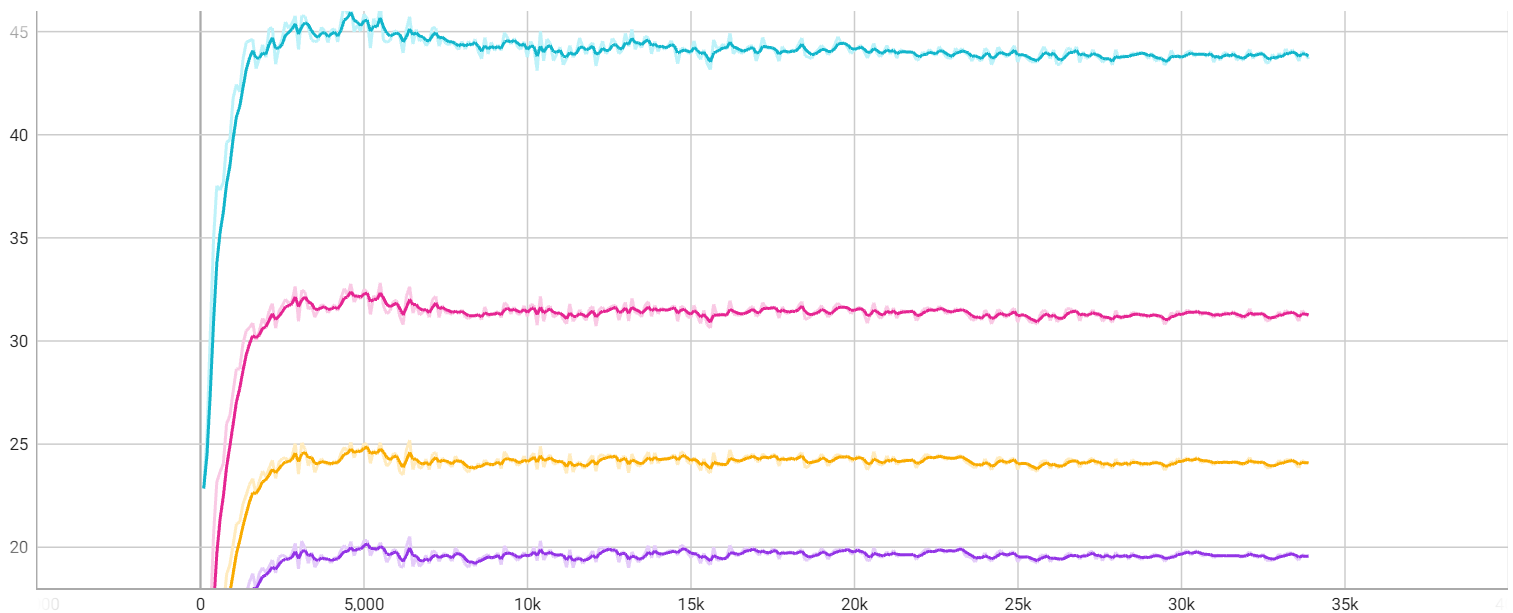
\includegraphics[width=1\textwidth]{../graphics/BlueScoresTraining.png}
    \caption{BLUE scores van het SignFormer model}
    \label{fig:blue-scores}

    \vspace{1cm}

    % Tweede figuur
    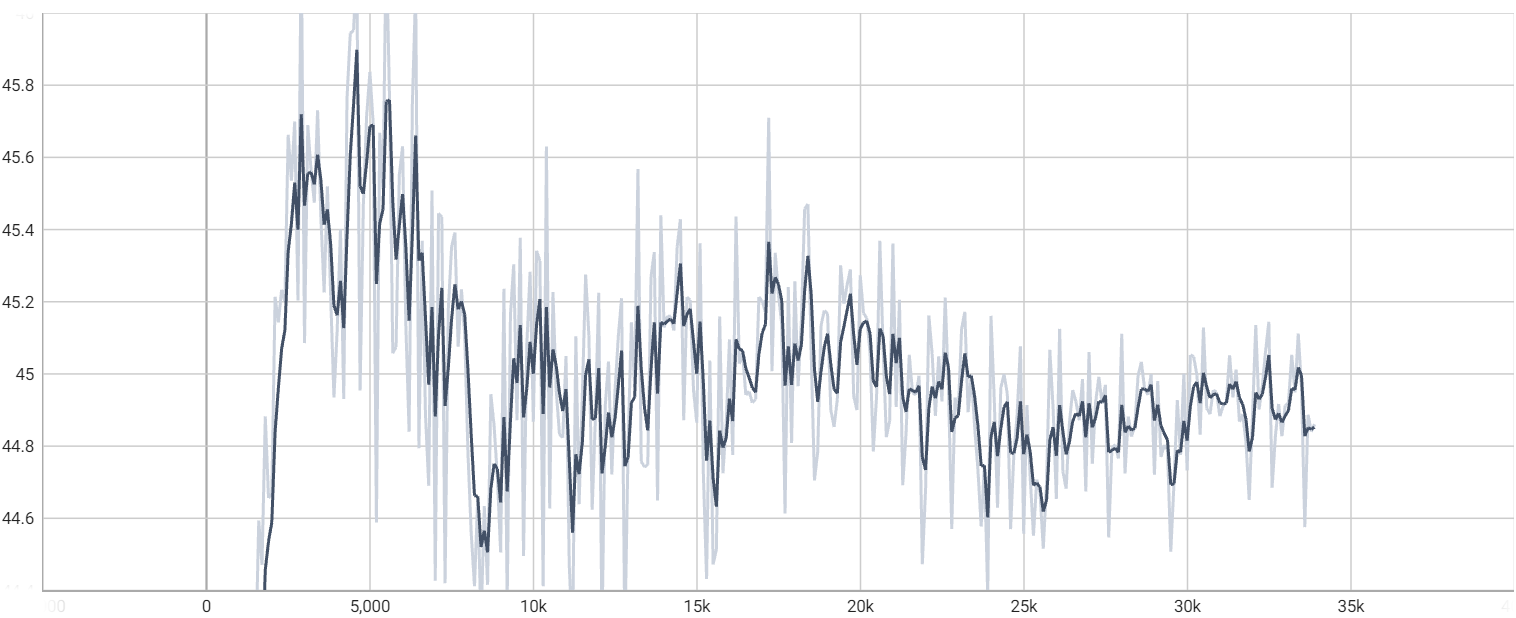
\includegraphics[width=1\textwidth]{../graphics/RougeScore.png}
    \caption{ROUGE scores van het SignFormer model}
    \label{fig:rouge-scores}

    \vspace{1cm} 

    % Derde figuur
    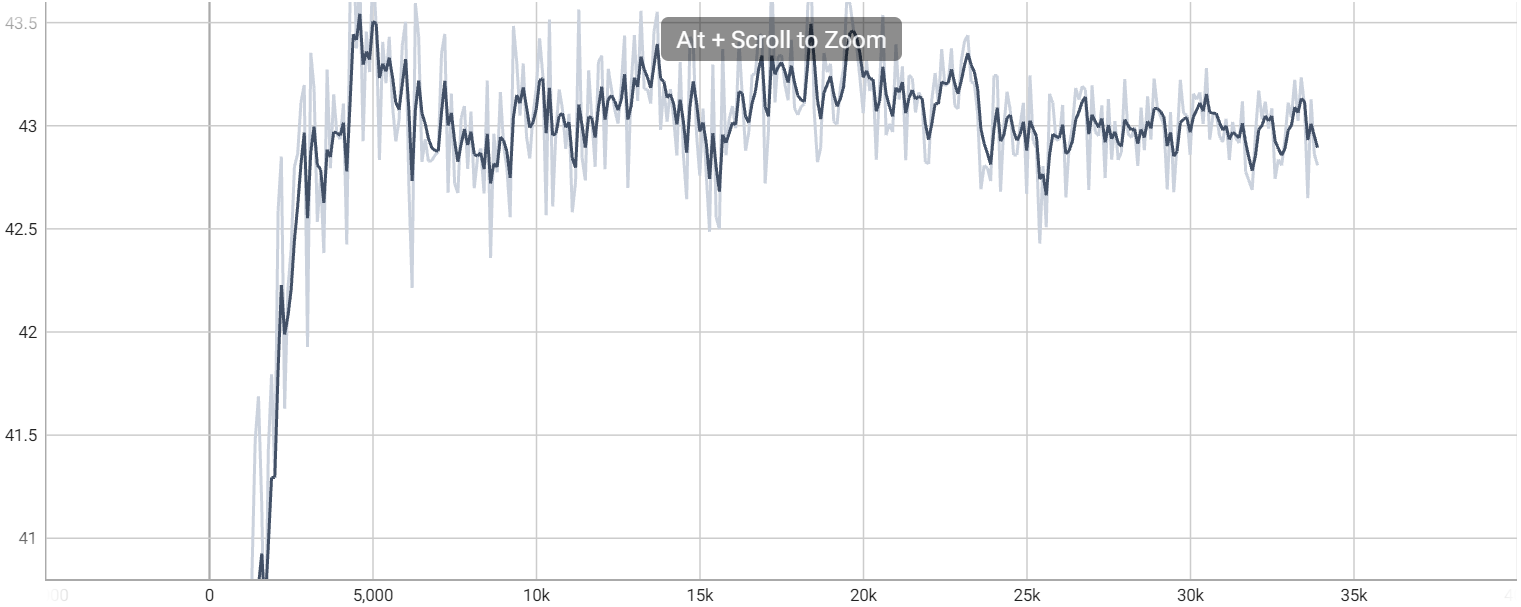
\includegraphics[width=1\textwidth]{../graphics/CHRF.png}
    \caption{CHRF scores van het SignFormer model}
    \label{fig:chrf-scores}
\end{figure}
